\documentclass[conference]{IEEEtran}
\usepackage{amsmath,amssymb,booktabs,graphicx,tikz}
\usepackage[T1]{fontenc}
\usepackage[hidelinks]{hyperref}
\title{Exact Adaptive DSP Packing for SNN Membrane Leakage}
\author{\IEEEauthorblockN{X}\IEEEauthorblockA{X}}
\begin{document}
\maketitle
\begin{abstract}
We present an exact FPGA leakage primitive whose actual membrane values select two narrow operations or one wide operation per DSP issue. Stored precision remains signed sixteen-bit and the declared result is $\lceil\beta U/256\rceil$ for unsigned Q8 coefficients $\beta\in[0,256]$. A compact overlapping layout uses a one-bit borrow reference and narrow rounded-result correction. The Artix-7 core includes admission and fallback in 62 LUTs, 44 FFs and one DSP, versus 202 LUTs and 79 FFs for fixed full-domain split packing at the same DSP budget. A public GLIF workload requires 46.01\% fewer issues than one-DSP scalar execution; a representative capture uses 12.37\% less estimated fixture dynamic energy. Against fixed split packing, estimated energy falls 60.95\% at a 1.08\% issue penalty. A two-DSP scalar pair remains near energy parity. Exhaustive arithmetic and fed-back public-model validation preserve the declared integer neuron exactly. Vanilla half-leakage shifting outperforms adaptation, delimiting its useful operating conditions.
\end{abstract}
\begin{IEEEkeywords}
DSP packing, spiking neural networks, membrane leakage, exact arithmetic, FPGA.
\end{IEEEkeywords}

\section{Introduction and Contribution}
Fixed-width neuron state must cover rare large membrane excursions, although many actual values are narrower. Packing based on this numerical range can improve DSP utilization without altering state precision. The circuit question is whether exact shared-coefficient leakage can cheaply admit narrow pairs while retaining the same wide legal input domain.

Value-dependent narrowness detection and operation packing are established~\cite{brooks}, as are signed DSP correction~\cite{dsppack}, exact spill reconstruction~\cite{wide} and runtime datatype packing~\cite{xtramac}. Our contribution is one integrated circuit mechanism: a compact exact rounded-leakage decoder, an actual-membrane pair/singleton contract, and its measured resource, issue-rate and estimated-energy trade-offs. It concerns leakage multiplication, rather than synaptic accumulation or a complete accelerator. It changes neither voltage units nor stored width, and introduces no mantissa/exponent scaling or packing approximation.

\section{Arithmetic and Admission Contract}
All general controls compute
\begin{equation}
 L(U,\beta)=\left\lceil\frac{\beta U}{256}\right\rceil,
 \quad U\in[-32768,32767],\quad\beta\in[0,256].
 \label{eq:leak}
\end{equation}
The result is signed sixteen-bit. A sufficiently wide signed numerator $\beta U+255$ followed by an arithmetic shift implements the ceiling for both signs. Saturation and wrapping are absent from the reference.

Two consecutive available operands are paired when both membranes fit $[-256,255]$ and their coefficients match. Otherwise the first is issued alone, retaining the next operand. Range tests, coefficient equality, arithmetic selection, correction and the returned consume count are inside the measured core. There is no externally supplied packing decision. A two-stage elastic valid/ready interface preserves order and held outputs under stalls.

The source advances by the returned count and re-presents unconsumed work. Source queues, operand memory and this variable-consumption integration are external. A stable common zero filter bypasses $U=0$ or $\beta=0$ in every scheduling control; its hardware is also excluded. Frame/window endpoints constrain pairing identically. Fig.~\ref{fig:datapath} distinguishes counted arithmetic from that external source.

\begin{figure}[t]
\centering
\resizebox{\columnwidth}{!}{%
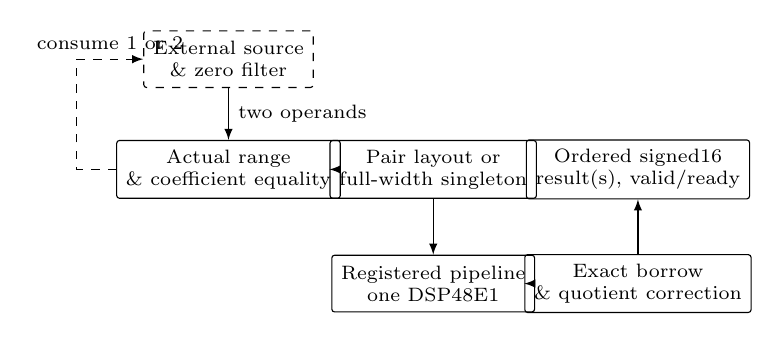
\begin{tikzpicture}[font=\scriptsize,>=latex,box/.style={draw,rounded corners=1pt,align=center,minimum width=2.15cm,minimum height=.72cm}]
\node[box,dashed] (src) at (0,2.25) {External source\\\& zero filter};
\node[box] (adm) at (0,.85) {Actual range\\\& coefficient equality};
\node[box] (lay) at (2.6,.85) {Pair layout or\\full-width singleton};
\node[box] (dsp) at (2.6,-.6) {Registered pipeline\\one DSP48E1};
\node[box] (dec) at (5.2,-.6) {Exact borrow\\\& quotient correction};
\node[box] (out) at (5.2,.85) {Ordered signed16\\result(s), valid/ready};
\draw[->] (src)--node[right]{two operands}(adm);
\draw[->] (adm)--(lay); \draw[->] (lay)--(dsp);
\draw[->] (dsp)--(dec); \draw[->] (dec)--(out);
\draw[->,dashed] (adm.west)--++(-.5,0)|-node[above,pos=.75]{consume 1 or 2}(src.west);
\end{tikzpicture}}
\caption{Counted E5 admission and arithmetic. The dashed source/filter is outside reported core area and energy. Unstalled latency is two advancing edges; no complete-neuron latency is claimed.}
\label{fig:datapath}
\end{figure}

\section{Exact Overlapping Leakage Decoder}
For an admitted pair $(u_0,u_1)$ and common coefficient, the DSP forms
\begin{align}
 A&=(u_0+256)+2^{16}u_1,\\
 C&=255-256\beta+255\,2^{16},\\
 P&=A\beta+C=x+2^{16}y,\label{eq:packed}
\end{align}
where $x=\beta u_0+255$ and $y=\beta u_1+255$. The multiplicand fits the signed twenty-five-bit DSP48E1 port. Since $-65536<x<65536$, its low field contributes either no spill or a single negative borrow $n=\mathbf1\{x<0\}$. Thus $T=\lfloor P/2^{16}\rfloor=y-n$.

Because $y$ has parity $r=(\beta_0\land(u_1)_0)\oplus1$, subtracting the borrow toggles the upper-field low bit. Therefore $n=P_{16}\oplus r$. Exact rounded results follow:
\begin{align}
 L_0&=\operatorname{uint}(P_{15:8})-256n,\label{eq:low}\\
 L_1&=\operatorname{int9}(P_{32:24})+
       \mathbf1\{n\land P_{23:16}=255\}.\label{eq:high}
\end{align}
Equation~\eqref{eq:low} restores the signed lower quotient; in~\eqref{eq:high}, adding the borrow changes the quotient only at the byte boundary. Results are sign-extended to sixteen bits. Coefficient endpoints $0,256$ and both membrane endpoints are covered. When admission fails, the same DSP executes an exact full-width singleton.

A straightforward nonoverlapping signed9 layout needs twenty-seven multiplicand bits at stride eighteen; restricting coefficients to this domain tightens that layout to twenty-six bits at stride seventeen. These are layout comparisons, not universal lower bounds. The same recovered borrow also reconstructs full products, so the distinction is economical rounded-output decoding, rather than unique feasibility of exact packing. Generic spill recovery is prior art~\cite{wide}.

\section{Matched Controls and Validation}
The primary one-DSP fixed control E1 decomposes $U=256h+q$, $0\le q\le255$:
\begin{equation}
 L(U,\beta)=\beta h+\left\lceil\beta q/256\right\rceil.
\end{equation}
Two residue products share a DSP; fabric forms two exact high contributions. E1 admits full-domain pairs when coefficients match. This ordinary quotient decomposition supplies a constructive baseline, not a separate novelty claim.

E3 uses two scalar DSPs, E4 one scalar DSP, and E7 an exact general LUT pair using floor quotient plus nonzero-remainder correction and a $\beta=256$ bypass. E6 is a zero-DSP half-leakage pair restricted to $\beta=128$. E9 is a shared zero-DSP add/sub pair restricted to all 33 trained GLIF coefficient codes (74--88 and 153--170), rather than one hardwired channel. All 2,162,688 signed16/code cases and the complete captured workload pass native RTL with and without stalls. E8 retains narrow packing on the same ports but removes range admission and full-width fallback; its caller must supply sign-extended signed9 operands. Thus E5--E8 measures combined admission/wide-support cost, not isolated controller area or a fair full-domain replacement.

Exhaustive checks cover 67,371,008 signed9 pair cases and 16,842,752 full-domain scalar/split cases without error. Native RTL checks cover 360,487 general operations per main engine with and without stalls, plus actual-model captures. Results, consumption, order and output holding match the independent integer reference; unstalled request latency is two advancing edges.

\subsection{Public Neuron Workloads}
Official GLIF ResNet18/CIFAR-10~\cite{glif} uses two time steps and channelwise coefficients. Integer membrane units are $1/256$ of source voltage units; effective leak coefficients are rounded nearest-even into Q8. Synapses and readout remain FP32. Previous-spike selection chooses one of two precomputed coefficients per channel; deferred reset and the source threshold comparison are preserved. The full 10,000-image scalar integer reference achieves 94.05\%, versus 94.03\% for the saved floating reference, with 371 changed predictions. This is conversion impact, not a packing accuracy gain. All 24,903,680,000 old/next states fit signed16. Packed feedback on 64 images matches every integer state/spike and final logit over 159,383,552 updates.

Official OTTT VGG11/CIFAR-10~\cite{ottt} uses six steps, $\tau=2$, and immediate subtractive reset. Its declared contract uses $L(U, 128)$ and threshold comparison $\ge256$. Full 10,000-image packed execution checks all 24,576,000,000 leakage updates independently with zero error. Floating accuracy is 93.49\%; integer/packed accuracy is 93.45\%, with 104 conversion-changed predictions. All observed stored states fit signed16. Exact shift leakage is consequently the required model-specific control.

An independent BNTT VGG11/TinyImageNet checkpoint~\cite{bntt} preserves thirty-step Poisson input, timestep normalization and deferred reset, with rounded $\beta=253$. On a predeclared 64-image held-out subset, packed and scalar integer states/spikes/logits agree over 1,171,783,680 updates; all stored states fit signed16. Floating/integer counts are 42/64 and 41/64, with one conversion-changed prediction. This is not full-test accuracy. Its exact constant alternative $L(U, 253)=U-\lfloor3U/256\rfloor$ passes all 65,536 scalar values; its hardware/energy remains unmeasured. AdEx is not evaluated.

\subsection{Route and Activity Protocol}
All controls target Artix-7 \texttt{xc7a100tcsg324-1}, Vivado 2025.2, a common 12~ns clock and falling-edge launch phase. Selected setup/hold checks pass. The common fixture has 94 FFs, excluded from core area but included in energy. No FMAX inference is made.

Accepted energy requires full known-pin replay under slow/max SDF with timing checks enabled and complete physical-net SAIF annotation. Unknown activity, partial intervals and unsupported defaults are rejected. Estimates are fixture dynamic energy at 25$^\circ$C, excluding chip static power, memory, full neuron integration and board power.

The predeclared representative GLIF capture uses seed 417839 and 2,176 stratified ordered contiguous windows, totaling 262,528 nonzero operands from the complete 64-image stream. Coefficient/membrane distribution and issue-overhead gates pass. OTTT uses 262,144 operands in 1,280 longer windows after retaining a failed short-window capture whose bias was traced to pairing restarts. Its unchanged distribution gates pass. These are bounded distribution-gated captures, not full-test energy or confidence intervals. All engines receive the same declared scalar operands within each comparison.

\section{Results and Operating Conditions}
Table~\ref{tab:results} reports selected matched routes and accepted energy. Admission and correction are included in E5's 62~LUT/44~FF/one DSP. Relative to E1, LUTs fall 69.31\% and FFs 44.30\%. E8's 47~LUT/36~FF/one DSP gives a combined 15~LUT/eight-FF admission/wide-support cost; its energy is unmeasured.

\begin{table}[t]
\centering\footnotesize
\caption{Core resources and accepted representative fixture dynamic energy (pJ/scalar). Common 94 fixture FFs excluded from area, included in energy. Separate GLIF/OTTT captures; dashes are unmeasured.}
\begin{tabular}{@{}lrrrrr@{}}
\toprule
Core&LUT&FF&DSP&GLIF&OTTT\\\midrule
E1 fixed split&202&79&1&55.308&36.808\\
E3 scalar pair&35&56&2&21.371&--\\
E4 scalar&13&29&1&24.648&--\\
E5 adaptive&62&44&1&21.599&26.580\\
E6 half shift&35&70&0&--&13.658\\
E7 LUT pair&330&88&0&124.198&--\\
E8 narrow only&47&36&1&--&--\\
E9 GLIF constants&375&82&0&96.758&--\\\bottomrule
\end{tabular}
\label{tab:results}
\end{table}

\begin{table}[t]
\centering\footnotesize
\caption{Complete evaluated stream issue counts after common zero filtering. GLIF/BNTT are 64-image streams; OTTT is the full 10,000-image test. Issues are not complete-neuron cycles.}
\begin{tabular}{@{}lrrr@{}}
\toprule
Stream&E5 issues&E1 issues&E5 penalty\\\midrule
GLIF&42,785,698&42,327,032&1.0836\%\\
OTTT&15,836,088,695&10,220,498,016&54.9444\%\\
BNTT&676,214,768&532,325,552&27.0303\%\\\bottomrule
\end{tabular}
\label{tab:issues}
\end{table}

In the complete GLIF stream, 99.0189\% of 79,246,135 nonzero operations fit signed9. E5 achieves 1.852 useful results per issue, 46.0091\% fewer issues than E4, and 1.0836\% more than E1 (Table~\ref{tab:issues}). Its representative energy is 12.3695\% below E4 while adding 49~LUT/15~FF. Against E1, energy falls 60.9472\% at a 1.0821\% captured issue penalty. E7 uses no DSP, but E5 reduces estimated energy 82.6089\% with 8.1148\% more captured issues. Against E3, DSP count halves while energy increases 1.0689\%: this is near energy parity and a resource trade-off, not superiority.

The GLIF capture contains 2,493 operands outside signed9. Deliberately unsafe wrapping changes every excluded leakage result: $(U,\beta)=(381,78)$ produces 117 correctly, versus $-39$ when forced to signed9. This establishes why narrow-only E8 cannot cover the unchanged workload; it is not a network-accuracy experiment.

Wider membrane profiles penalize adaptation. Representative OTTT E5 saves 27.7876\% energy versus general E1 but consumes 94.6139\% more than exact half-leakage shifting. Full OTTT issues increase 54.9444\% versus E1; BNTT increases 27.0303\%. All-wide same-coefficient bursts favor E1, and coefficient mismatch prevents pairing in both. Universal burst-latency improvement is not claimed. The shared 33-code GLIF constant control E9 uses 375~LUT/82~FF/zero DSP and 96.758~pJ/scalar on the same capture. This measured add/sub construction is one checkpoint-restricted alternative, not an optimality bound for specialized constants.

Twelve of fourteen planned GLIF/retained-OTTT-stress energy controls passed. Original LUT E2 delayed replay failed and supplies no energy. Its timed CARRY4 discrepancy remains diagnostic, not accepted energy. E7 independently passes full delayed replay and activity audit, preserving the accepted fabric comparison. Raw failed evidence and the detailed diagnostic remain retained.

\section{Related Work and Conclusion}
FireFly~\cite{firefly} uses fixed twelve-bit SIMD accumulation and shift-based $\tau=2$ leakage. Its complete accelerator metrics are not comparable to our leakage issues/fixture energy. Our constructed fixed and LUT controls reproduce the same arithmetic operation, rather than FireFly's accelerator.

UDP's complete methods~\cite{udp} configure widths and parallelism before hardware generation, with runtime sign/most-negative corrections and high/low fusion. They do not describe this membrane pair/singleton policy. Ou's dynamic packing~\cite{ou}, Cui's lossless signed packing~\cite{cui} and McKeown's range utilization~\cite{mckeown} are relevant; their original full methods remain unavailable in this bounded review. We therefore claim the specific implemented leakage mechanism and measured trade-offs, rather than proven absence or generic first-ever packing. Existing range detection and spill arithmetic are explicitly credited.

The exact decoder and membrane admission provide a compact one-DSP alternative at unchanged signed16 precision. Public-model checks support integer exactness, and matched measurements expose positive GLIF trade-offs alongside constant-leakage negative cases. External source integration, further constant optimization and three uninspected methods delimit the result; this is a leakage primitive contribution, not a complete SNN accelerator or an accuracy improvement.

\section*{Acknowledgment}
OpenAI Codex assisted with RTL/software prototyping, validation tooling, evidence analysis, and drafting the abstract, Fig.~\ref{fig:datapath} and Sections I--VI. Reported measurements derive from preserved tool/model executions.

% Enforce four technical pages without changing IEEE font sizes or margins.
\clearpage
\ifnum\value{page}>5
\PackageError{manuscript}{Technical content exceeds four pages}{Shorten technical content; retain IEEE template dimensions.}
\fi
\begin{thebibliography}{99}
\bibitem{brooks} D. Brooks and M. Martonosi, ``Value-Based Clock Gating and Operation Packing: Dynamic Strategies for Improving Processor Power and Performance,'' \emph{ACM TOCS}, vol.18, no.2, pp.89--126, 2000, doi:10.1145/350853.350856.
\bibitem{dsppack} J. Sommer, A. Ozkan, O. Keszocze and J. Teich, ``DSP-Packing: Squeezing Low-precision Arithmetic into FPGA DSP Blocks,'' FPL 2022, arXiv:2203.11028.
\bibitem{wide} T. Borntrager et al., ``Arithmetic Packing on Wide Integer Datapaths in DSP Primitives of Modern FPGA Devices,'' 2026, arXiv:2606.11065.
\bibitem{xtramac} F. Yu et al., ``XtraMAC: An Efficient MAC Architecture for Mixed-Precision LLM Inference on FPGA,'' 2026, arXiv:2605.06052.
\bibitem{firefly} J. Li, G. Shen, D. Zhao, Q. Zhang and Y. Zeng, ``FireFly: A High-Throughput Hardware Accelerator for Spiking Neural Networks With Efficient DSP and Memory Optimization,'' \emph{IEEE Trans. VLSI Syst.}, vol.31, no.8, pp.1178--1191, Aug. 2023, doi:10.1109/TVLSI.2023.3279349.
\bibitem{glif} X. Yao, F. Li, Z. Mo and J. Cheng, ``GLIF: A Unified Gated Leaky Integrate-and-Fire Neuron for Spiking Neural Networks,'' \emph{Advances in Neural Information Processing Systems}, vol.35, pp.32160--32171, 2022. Official code: \url{https://github.com/CAS-CLab/Gated-LIF}.
\bibitem{ottt} M. Xiao, Q. Meng, Z. Zhang, D. He and Z. Lin, ``Online Training Through Time for Spiking Neural Networks,'' \emph{Advances in Neural Information Processing Systems}, vol.35, pp.20717--20730, 2022. Official code: \url{https://github.com/pkuxmq/OTTT-SNN}.
\bibitem{bntt} Y. Kim and P. Panda, ``Visual explanations from spiking neural networks using inter-spike intervals,'' \emph{Scientific Reports}, vol.11, art.19037, 2021, doi:10.1038/s41598-021-98448-0.
\bibitem{udp} J. Wu, Z. Zheng, L. Gong, C. Wang and X. Zhou, ``UDP: A Universal DSP Packing Framework for Low-bitwidth MAC Acceleration on FPGAs,'' FPGA 2026, pp.212--223, doi:10.1145/3748173.3779194.
\bibitem{ou} Y. Ou et al., ``A 119.64 GOPs/W FPGA-Based ResNet50 Mixed-Precision Accelerator Using the Dynamic DSP Packing,'' \emph{IEEE TCAS-II}, vol.71, no.5, pp.2554--2558, 2024, doi:10.1109/TCSII.2024.3377356.
\bibitem{cui} Z. Cui et al., ``Efficient DSP Packing Method for Neural Network Accelerator,'' ICFPT 2024, doi:10.1109/ICFPT64416.2024.11113473.
\bibitem{mckeown} S. McKeown, R. Woods and J. McAllister, ``Power efficient dynamic-range utilisation for DSP on FPGA,'' SIPS 2008, pp.233--238, doi:10.1109/SIPS.2008.4671768.
\end{thebibliography}
\ifnum\value{page}>5
\PackageError{manuscript}{Total content exceeds five pages}{Shorten references to fit the optional fifth page.}
\fi
\end{document}
